% Created 2018-12-12 Wed 10:33
% Intended LaTeX compiler: pdflatex
\documentclass[11pt]{article}
\usepackage[utf8]{inputenc}
\usepackage[T1]{fontenc}
\usepackage{graphicx}
\usepackage{grffile}
\usepackage{longtable}
\usepackage{wrapfig}
\usepackage{rotating}
\usepackage[normalem]{ulem}
\usepackage{amsmath}
\usepackage{textcomp}
\usepackage{amssymb}
\usepackage{capt-of}
\usepackage{hyperref}
\usepackage{minted}
\usepackage[1.0in]{geometry}
\author{Mijeong Ban}
\date{\today}
\title{}
\hypersetup{
 pdfauthor={Mijeong Ban},
 pdftitle={},
 pdfkeywords={},
 pdfsubject={},
 pdfcreator={Emacs 26.1 (Org mode 9.1.9)}, 
 pdflang={English}}
\begin{document}


\section*{Part One. Statistical Report}
\label{sec:org3cfe7e7}

\section*{Part Two. Textbook Exercises}
\label{sec:org27e6fdb}
\subsection*{11.42 Relationships among PCB congeners}
\label{sec:orgd2076a7}
Consider the following variables: PCB(the total amount of PCB) and four congeners: PCB52, PCB118, PCB138, and PCB180.
\subsubsection*{(a) Using numerical and graphical summaries, describe the distribution of each of these variables.}
\label{sec:org2dcda17}
\begin{table}[htbp]
\caption{Numerical Summaries}
\centering
\begin{tabular}{lrrrrrr}
Variable & Min & 1st Qu. & Median & Mean & 3rd Qu. & Max\\
\hline
PCB & 6.10 & 30.18 & 47.96 & 68.47 & 91.63 & 318.70\\
PCB52 & 0.020 & 0.228 & 0.477 & 0.958 & 0.892 & 9.060\\
PCB118 & 0.236 & 1.490 & 2.420 & 3.256 & 3.890 & 18.900\\
PCB138 & 0.640 & 3.180 & 4.920 & 6.827 & 8.650 & 32.300\\
PCB180 & 0.395 & 1.240 & 2.690 & 4.158 & 4.490 & 31.500\\
\end{tabular}
\end{table}

\begin{figure}[htbp]
\centering
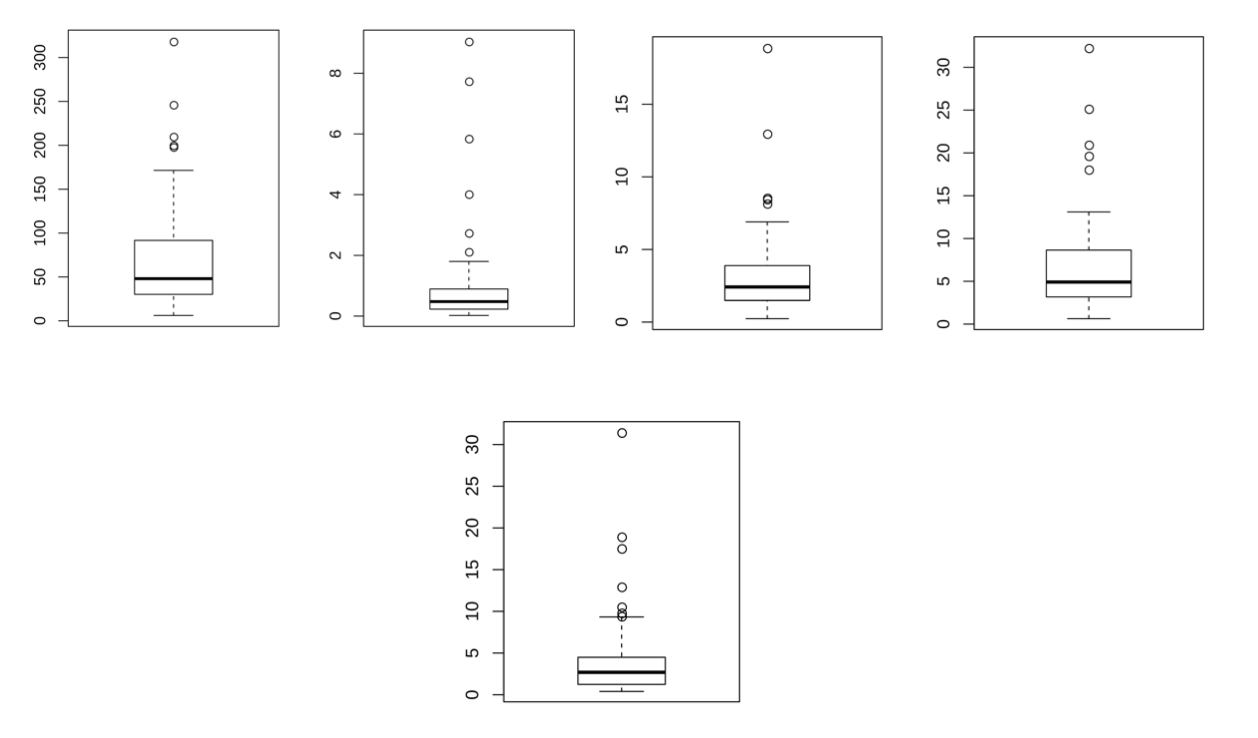
\includegraphics[width=.9\linewidth]{./graphs/image1.png}
\caption{Boxplots of PCB, PBC52, PCB118, PCB138 and PCB180}
\end{figure}
Figure 1 shows that the distribution of PCB and PCB180 is right skewed with about six outliers for both, while all the distribution of others are right skewed with about five outliers.  

\subsubsection*{(b) Using numerical and graphical summaries, describe the relationship between each pair of variables.}
\label{sec:org8456440}
\begin{table}[htbp]
\caption{Correlations}
\centering
\begin{tabular}{llr}
Variable 1 & Variable 2 & Correlation\\
\hline
PCB & PCB52 & 0.5963572\\
PCB & PCB118 & 0.843298\\
PCB & PCB138 & 0.9288353\\
PCB & PCB180 & 0.8008549\\
PCB52 & PCB118 & 0.6849073\\
PCB52 & PCB138 & 0.3008983\\
PCB52 & PCB180 & 0.08692971\\
PCB118 & PCB138 & 0.7293792\\
PCB118 & PCB180 & 0.4374443\\
PCB138 & PCB180 & 0.8823022\\
\end{tabular}
\end{table}

\begin{center}
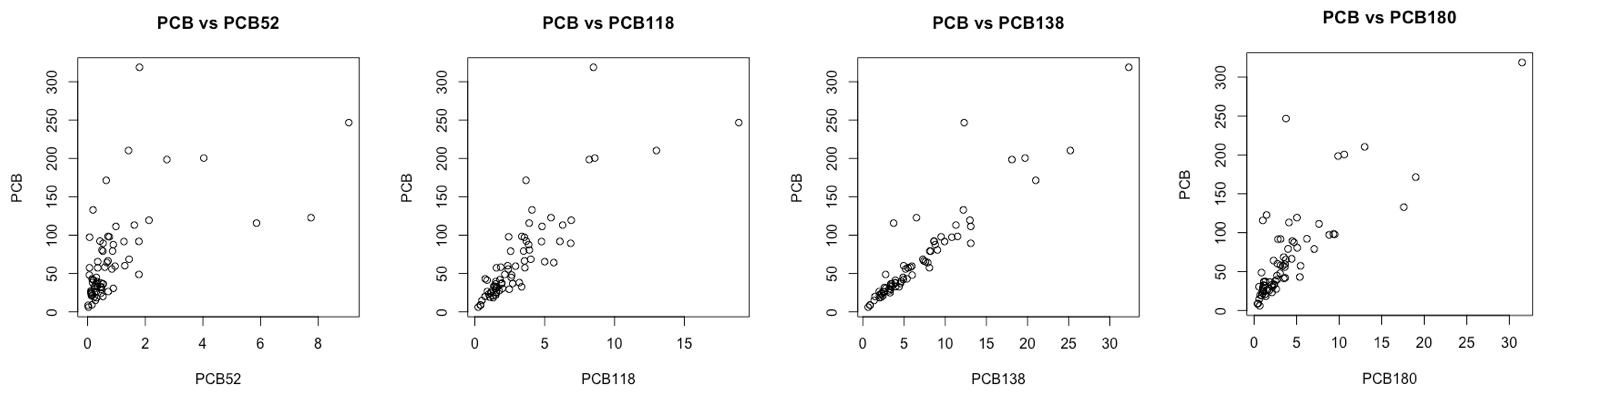
\includegraphics[width=.9\linewidth]{./graphs/image2.png}
\end{center}
\begin{center}
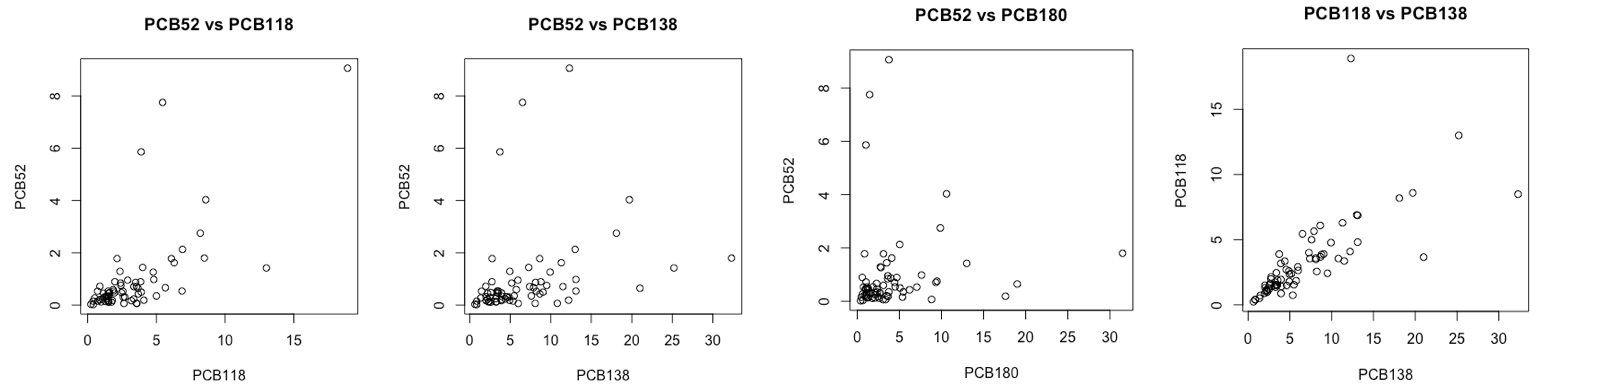
\includegraphics[width=.9\linewidth]{./graphs/image3.png}
\end{center}
\begin{center}
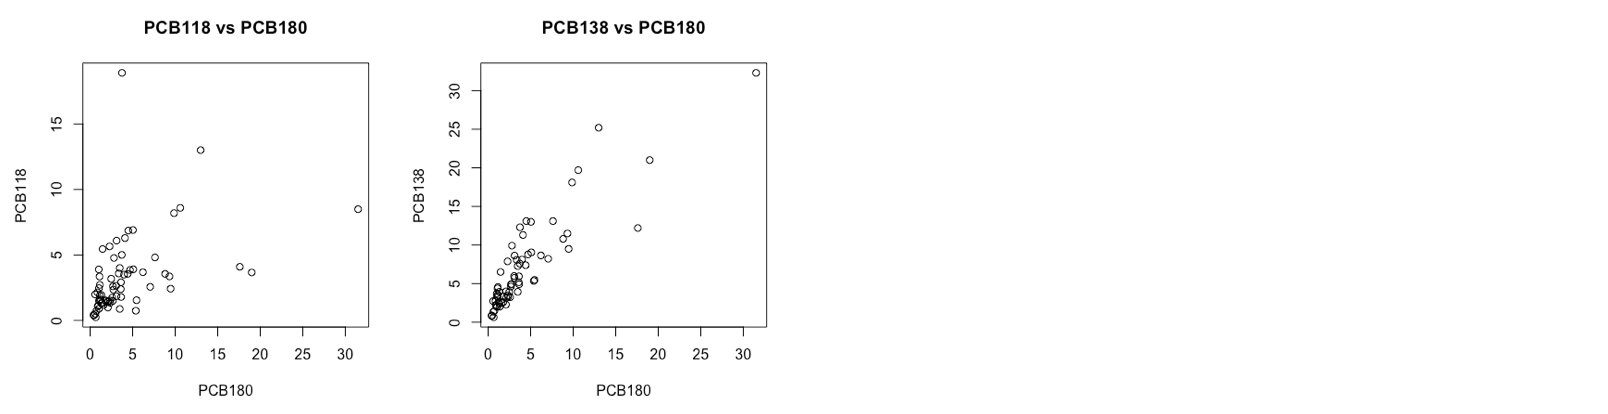
\includegraphics[width=.9\linewidth]{./graphs/image4.png}
\end{center}

\subsection*{11.43 Predictiong the total amount of PCB}
\label{sec:org86e63f7}
Use the four congeners PCB52, PCB118, PCB138, and PCB180 in a multiple regression to predict PCB. 
\subsubsection*{(a) Write the statistical model for this analysis. Include all assumptions.}
\label{sec:org0676b31}
The multiple linear regression model for the data with 69 observations:

y\(_{\text{i}}\) = \(\beta_{\text{0}}\) + \(\beta_{\text{1}}\)x\(_{\text{i1}}\) + \(\beta_{\text{2}}\)x\(_{\text{i2}}\) + \(\beta_{\text{3}}\)x\(_{\text{i3}}\) + \(\beta_{\text{4}}\)x\(_{\text{i4}}\) + i \emph{for} \emph{i = 1, 2, \ldots{} , 69}

We assume that the residuals are independent and are normally distributed. 
\subsubsection*{(b) Run the regression and summarize the results.}
\label{sec:org48427f9}
Multiple regression analyses were conducted to examine the relationship between PCB and four congeners. Running the multiple regression model in R with the four congeners produced the following:
\begin{verbatim}

subdf <- subset(df, select = c("pcb", "pcb52", "pcb118", "pcb138", "pcb180"))
> lm1 = lm(pcb~pcb52 + pcb118 + pcb138 + pcb180, data=subdf)
> coef(lm1)
(Intercept)       pcb52      pcb118      pcb138      pcb180 
  0.9369203  11.8726953   3.7610694   3.8842264   4.1823010 
> summary(lm1)

Call:
lm(formula = pcb ~ pcb52 + pcb118 + pcb138 + pcb180, data = subdf)

Residuals:
     Min       1Q   Median       3Q      Max 
-22.0864  -2.4554   0.0278   2.7726  22.5487 

Coefficients:
            Estimate Std. Error t value Pr(>|t|)    
(Intercept)   0.9369     1.2293   0.762    0.449    
pcb52        11.8727     0.7290  16.287  < 2e-16 ***
pcb118        3.7611     0.6424   5.855 1.79e-07 ***
pcb138        3.8842     0.4978   7.803 7.19e-11 ***
pcb180        4.1823     0.4318   9.687 3.64e-14 ***
---
Signif. codes:  0 ‘***’ 0.001 ‘**’ 0.01 ‘*’ 0.05 ‘.’ 0.1 ‘ ’ 1

Residual standard error: 6.382 on 64 degrees of freedom
Multiple R-squared:  0.9891,	Adjusted R-squared:  0.9885 
F-statistic:  1456 on 4 and 64 DF,  p-value: < 2.2e-16

> anova(lm1)
Analysis of Variance Table

Response: pcb
          Df Sum Sq Mean Sq  F value    Pr(>F)    
pcb52      1  85302   85302 2094.273 < 2.2e-16 ***
pcb118     1  85429   85429 2097.405 < 2.2e-16 ***
pcb138     1  62693   62693 1539.202 < 2.2e-16 ***
pcb180     1   3822    3822   93.834  3.64e-14 ***
Residuals 64   2607      41                       
---
Signif. codes:  0 ‘***’ 0.001 ‘**’ 0.01 ‘*’ 0.05 ‘.’ 0.1 ‘ ’ 1
\end{verbatim}
\begin{itemize}
\item We gathered the following from the results of the regression:
\label{sec:org509e1e0}
\begin{itemize}
\item The multiple R\(^{\text{2}}\) = 0.989
\item The residual SE = 6.249
\end{itemize}
\end{itemize}

\item Test 1
\label{sec:org2673595}

H\(_{\text{0}}\) : \(\beta_{\text{0}}\) = \(\beta_{\text{1}}\) = \(\beta_{\text{2}}\) = \(\beta_{\text{3}}\) = \(\beta_{\text{4}}\) = 0

H\(_{\text{1}}\) : \(\beta_{\text{0}}\) \(\neq\) 0 \(\vee\) \(\beta_{\text{1}}\) \(\neq\) 0 \(\vee\) \(\beta_{\text{2}}\) \(\neq\) 0 \(\vee\) \(\beta_{\text{3}}\) \(\neq\) 0 \(\vee\) \(\beta_{\text{4}}\) \(\neq\) 0

Since there is at least one \(\beta_{\text{n}}\) \(\neq\) 0, we reject H\(_{\text{0}}\) 

\item Test 2
\label{sec:org7c7d28c}

H\(_{\text{0}}\) = \(\beta_{\text{j}}\) = 0, \emph{j = 0, 1, 2, 3}

H\(_{\text{1}}\) = \(\beta_{\text{j}}\) \(\neq\) 0

All regression coefficients are significantly different from 0 with the except of 0.94. We found that R\(^{\text{2}}\) = 0.989, meaning that 98.9\% of variation in PCB is from PCB52, PCB118, PCB138 and PCB180.
\end{itemize}

\subsubsection*{(c) Examine the residuals. Do they appear to be approximately Normal? When you plot them versus each of the explanatory variables, are any patterns evident?}
\label{sec:org0ef6630}
\begin{center}
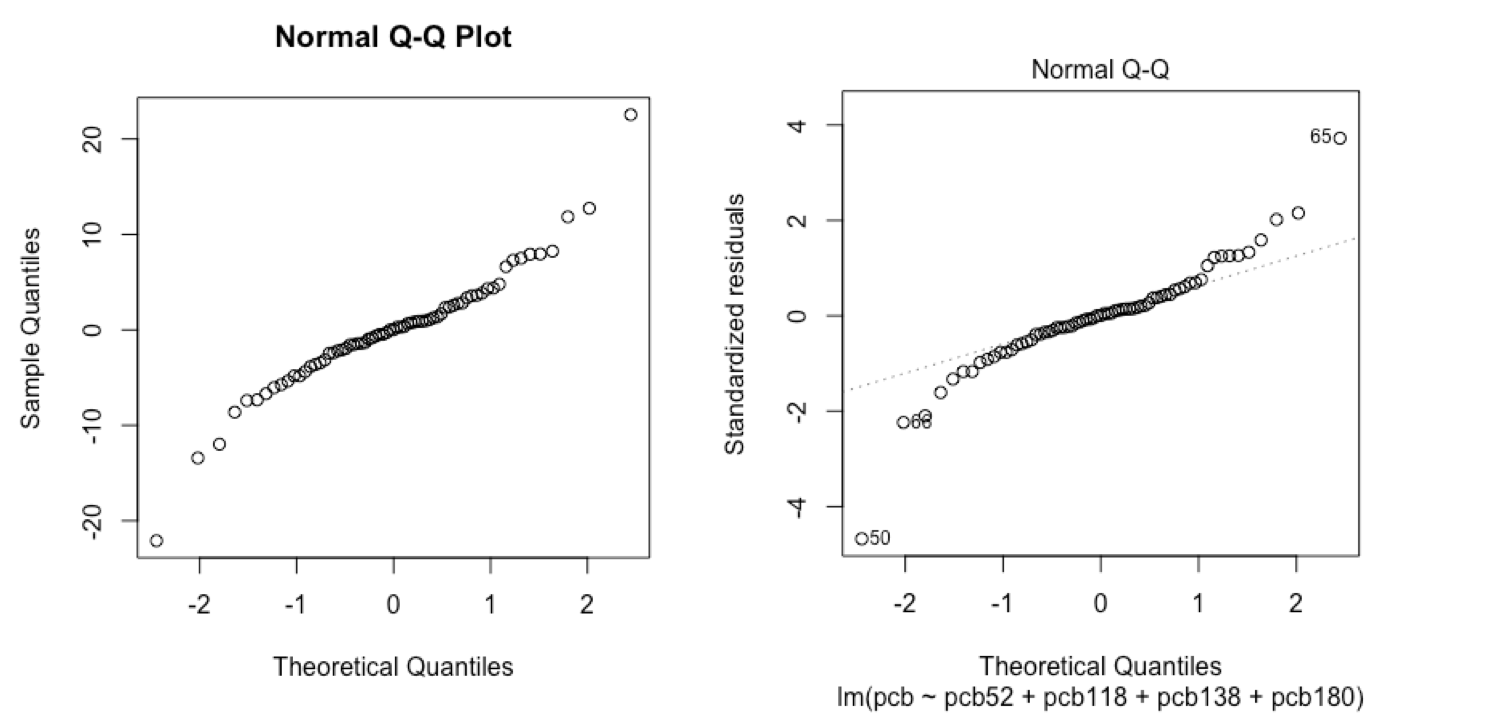
\includegraphics[width=.9\linewidth]{./graphs/image5.png}
\end{center}
According to the graphs, the residuals shows two clear outliers and shows that the residuals are approximately normal. Rhere are no other patterns in the explanatory variables of note. 

\subsection*{11.44 Adjusting the analysis for potential outliers.}
\label{sec:orgcebf3fd}
The examination of 
\end{document}
